% Options for packages loaded elsewhere
\PassOptionsToPackage{unicode}{hyperref}
\PassOptionsToPackage{hyphens}{url}
%
\documentclass[
]{book}
\usepackage{lmodern}
\usepackage{amssymb,amsmath}
\usepackage{ifxetex,ifluatex}
\ifnum 0\ifxetex 1\fi\ifluatex 1\fi=0 % if pdftex
  \usepackage[T1]{fontenc}
  \usepackage[utf8]{inputenc}
  \usepackage{textcomp} % provide euro and other symbols
\else % if luatex or xetex
  \usepackage{unicode-math}
  \defaultfontfeatures{Scale=MatchLowercase}
  \defaultfontfeatures[\rmfamily]{Ligatures=TeX,Scale=1}
\fi
% Use upquote if available, for straight quotes in verbatim environments
\IfFileExists{upquote.sty}{\usepackage{upquote}}{}
\IfFileExists{microtype.sty}{% use microtype if available
  \usepackage[]{microtype}
  \UseMicrotypeSet[protrusion]{basicmath} % disable protrusion for tt fonts
}{}
\makeatletter
\@ifundefined{KOMAClassName}{% if non-KOMA class
  \IfFileExists{parskip.sty}{%
    \usepackage{parskip}
  }{% else
    \setlength{\parindent}{0pt}
    \setlength{\parskip}{6pt plus 2pt minus 1pt}}
}{% if KOMA class
  \KOMAoptions{parskip=half}}
\makeatother
\usepackage{xcolor}
\IfFileExists{xurl.sty}{\usepackage{xurl}}{} % add URL line breaks if available
\IfFileExists{bookmark.sty}{\usepackage{bookmark}}{\usepackage{hyperref}}
\hypersetup{
  pdftitle={Reproducible Science Project},
  pdfauthor={Sara Wall},
  hidelinks,
  pdfcreator={LaTeX via pandoc}}
\urlstyle{same} % disable monospaced font for URLs
\usepackage{color}
\usepackage{fancyvrb}
\newcommand{\VerbBar}{|}
\newcommand{\VERB}{\Verb[commandchars=\\\{\}]}
\DefineVerbatimEnvironment{Highlighting}{Verbatim}{commandchars=\\\{\}}
% Add ',fontsize=\small' for more characters per line
\usepackage{framed}
\definecolor{shadecolor}{RGB}{248,248,248}
\newenvironment{Shaded}{\begin{snugshade}}{\end{snugshade}}
\newcommand{\AlertTok}[1]{\textcolor[rgb]{0.94,0.16,0.16}{#1}}
\newcommand{\AnnotationTok}[1]{\textcolor[rgb]{0.56,0.35,0.01}{\textbf{\textit{#1}}}}
\newcommand{\AttributeTok}[1]{\textcolor[rgb]{0.77,0.63,0.00}{#1}}
\newcommand{\BaseNTok}[1]{\textcolor[rgb]{0.00,0.00,0.81}{#1}}
\newcommand{\BuiltInTok}[1]{#1}
\newcommand{\CharTok}[1]{\textcolor[rgb]{0.31,0.60,0.02}{#1}}
\newcommand{\CommentTok}[1]{\textcolor[rgb]{0.56,0.35,0.01}{\textit{#1}}}
\newcommand{\CommentVarTok}[1]{\textcolor[rgb]{0.56,0.35,0.01}{\textbf{\textit{#1}}}}
\newcommand{\ConstantTok}[1]{\textcolor[rgb]{0.00,0.00,0.00}{#1}}
\newcommand{\ControlFlowTok}[1]{\textcolor[rgb]{0.13,0.29,0.53}{\textbf{#1}}}
\newcommand{\DataTypeTok}[1]{\textcolor[rgb]{0.13,0.29,0.53}{#1}}
\newcommand{\DecValTok}[1]{\textcolor[rgb]{0.00,0.00,0.81}{#1}}
\newcommand{\DocumentationTok}[1]{\textcolor[rgb]{0.56,0.35,0.01}{\textbf{\textit{#1}}}}
\newcommand{\ErrorTok}[1]{\textcolor[rgb]{0.64,0.00,0.00}{\textbf{#1}}}
\newcommand{\ExtensionTok}[1]{#1}
\newcommand{\FloatTok}[1]{\textcolor[rgb]{0.00,0.00,0.81}{#1}}
\newcommand{\FunctionTok}[1]{\textcolor[rgb]{0.00,0.00,0.00}{#1}}
\newcommand{\ImportTok}[1]{#1}
\newcommand{\InformationTok}[1]{\textcolor[rgb]{0.56,0.35,0.01}{\textbf{\textit{#1}}}}
\newcommand{\KeywordTok}[1]{\textcolor[rgb]{0.13,0.29,0.53}{\textbf{#1}}}
\newcommand{\NormalTok}[1]{#1}
\newcommand{\OperatorTok}[1]{\textcolor[rgb]{0.81,0.36,0.00}{\textbf{#1}}}
\newcommand{\OtherTok}[1]{\textcolor[rgb]{0.56,0.35,0.01}{#1}}
\newcommand{\PreprocessorTok}[1]{\textcolor[rgb]{0.56,0.35,0.01}{\textit{#1}}}
\newcommand{\RegionMarkerTok}[1]{#1}
\newcommand{\SpecialCharTok}[1]{\textcolor[rgb]{0.00,0.00,0.00}{#1}}
\newcommand{\SpecialStringTok}[1]{\textcolor[rgb]{0.31,0.60,0.02}{#1}}
\newcommand{\StringTok}[1]{\textcolor[rgb]{0.31,0.60,0.02}{#1}}
\newcommand{\VariableTok}[1]{\textcolor[rgb]{0.00,0.00,0.00}{#1}}
\newcommand{\VerbatimStringTok}[1]{\textcolor[rgb]{0.31,0.60,0.02}{#1}}
\newcommand{\WarningTok}[1]{\textcolor[rgb]{0.56,0.35,0.01}{\textbf{\textit{#1}}}}
\usepackage{longtable,booktabs}
% Correct order of tables after \paragraph or \subparagraph
\usepackage{etoolbox}
\makeatletter
\patchcmd\longtable{\par}{\if@noskipsec\mbox{}\fi\par}{}{}
\makeatother
% Allow footnotes in longtable head/foot
\IfFileExists{footnotehyper.sty}{\usepackage{footnotehyper}}{\usepackage{footnote}}
\makesavenoteenv{longtable}
\usepackage{graphicx,grffile}
\makeatletter
\def\maxwidth{\ifdim\Gin@nat@width>\linewidth\linewidth\else\Gin@nat@width\fi}
\def\maxheight{\ifdim\Gin@nat@height>\textheight\textheight\else\Gin@nat@height\fi}
\makeatother
% Scale images if necessary, so that they will not overflow the page
% margins by default, and it is still possible to overwrite the defaults
% using explicit options in \includegraphics[width, height, ...]{}
\setkeys{Gin}{width=\maxwidth,height=\maxheight,keepaspectratio}
% Set default figure placement to htbp
\makeatletter
\def\fps@figure{htbp}
\makeatother
\setlength{\emergencystretch}{3em} % prevent overfull lines
\providecommand{\tightlist}{%
  \setlength{\itemsep}{0pt}\setlength{\parskip}{0pt}}
\setcounter{secnumdepth}{5}
\usepackage{booktabs}
\usepackage[]{natbib}
\bibliographystyle{apalike}

\title{Reproducible Science Project}
\author{Sara Wall}
\date{2021-03-08}

\begin{document}
\maketitle

{
\setcounter{tocdepth}{1}
\tableofcontents
}
\hypertarget{introduction}{%
\chapter{Introduction}\label{introduction}}

This book is the final project for WILD6900. The book contains work and data from my MS thesis on post-fire debris flows.

\hypertarget{database}{%
\chapter{Create Database}\label{database}}

This document will create a database for my MS Research Data.

The database will follow the following structure:

\begin{figure}

{\centering 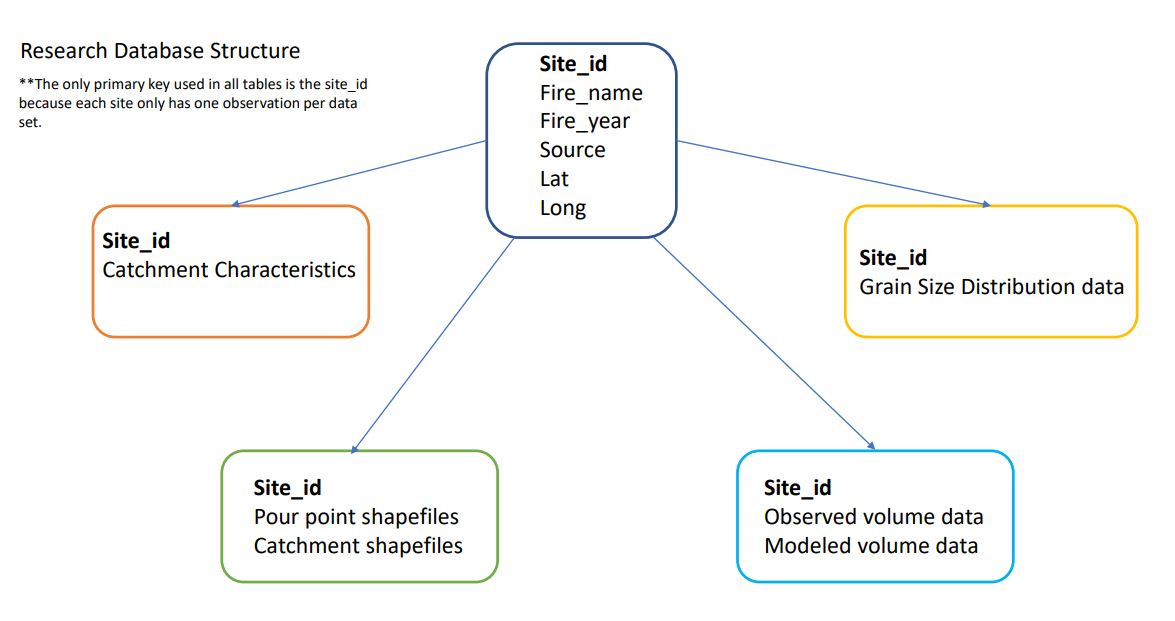
\includegraphics[width=0.8\linewidth]{database_structure} 

}

\caption{Database Structure}\label{fig:image}
\end{figure}

The data in this database is compiled from primary fieldwork and from data found in the literature. For each post-fire debris flow characterized, location, grain size, volume, and catchment characteristics are provided. Each debris flow fan is characterized once and therefore the site\_id for each fan is used as the Primary Key in all data sets in the database.

\hypertarget{step-1.-load-packages-and-connect-to-the-sql-database}{%
\section{Step 1. Load packages and connect to the SQL database}\label{step-1.-load-packages-and-connect-to-the-sql-database}}

\begin{Shaded}
\begin{Highlighting}[]
\CommentTok{# Load packages ####}

\KeywordTok{library}\NormalTok{(DBI)}
\KeywordTok{library}\NormalTok{(RSQLite)}
\end{Highlighting}
\end{Shaded}

\begin{verbatim}
## Warning: package 'RSQLite' was built under R version 4.0.3
\end{verbatim}

\begin{Shaded}
\begin{Highlighting}[]
\KeywordTok{library}\NormalTok{(rlang)}
\end{Highlighting}
\end{Shaded}

\begin{verbatim}
## Warning: package 'rlang' was built under R version 4.0.3
\end{verbatim}

\begin{Shaded}
\begin{Highlighting}[]
\CommentTok{# Establish database connection ####}

\NormalTok{debrisflow_db <-}\StringTok{ }\KeywordTok{dbConnect}\NormalTok{(}\DataTypeTok{drv =}\NormalTok{ RSQLite}\OperatorTok{::}\KeywordTok{SQLite}\NormalTok{(), }\StringTok{"database/MS_research_db.db"}\NormalTok{)}
\end{Highlighting}
\end{Shaded}

\hypertarget{step-2.-create-df_locations-table}{%
\section{Step 2. Create DF\_Locations Table}\label{step-2.-create-df_locations-table}}

\begin{Shaded}
\begin{Highlighting}[]
\KeywordTok{dbExecute}\NormalTok{(debrisflow_db, }\StringTok{"CREATE TABLE DF_locations (}
\StringTok{          Site_id varchar(50),}
\StringTok{          Fire varchar(50),}
\StringTok{          fire_year varchar(5),}
\StringTok{          Source varchar(50),}
\StringTok{          year_surveyed varchar(5),}
\StringTok{          Lat double,}
\StringTok{          long double, PRIMARY KEY (Site_id));}
\StringTok{          "}\NormalTok{)}

\NormalTok{DF_locations <-}\StringTok{ }\KeywordTok{read.csv}\NormalTok{(}\StringTok{"DF_locations.csv"}\NormalTok{, }\DataTypeTok{header =} \OtherTok{TRUE}\NormalTok{, }\DataTypeTok{stringsAsFactors =} \OtherTok{FALSE}\NormalTok{)}

\KeywordTok{names}\NormalTok{(DF_locations)}

\KeywordTok{dbWriteTable}\NormalTok{(debrisflow_db, }\StringTok{"DF_locations"}\NormalTok{, DF_locations, }\DataTypeTok{append=} \OtherTok{TRUE}\NormalTok{)}
\end{Highlighting}
\end{Shaded}

\begin{Shaded}
\begin{Highlighting}[]
\CommentTok{#Check table}
\KeywordTok{dbGetQuery}\NormalTok{(debrisflow_db, }\StringTok{"SELECT * FROM DF_locations LIMIT 10;"}\NormalTok{)}
\end{Highlighting}
\end{Shaded}

\begin{verbatim}
##           Site_id              Fire fire_year            Source year_surveyed
## 1     Brianhead 1         Brianhead      2017 Primary Fieldwork          2020
## 2     Brianhead 2         Brianhead      2017 Primary Fieldwork          2020
## 3     Brianhead 3         Brianhead      2017 Primary Fieldwork          2020
## 4   Brianhead 3.2         Brianhead      2017 Primary Fieldwork          2020
## 5     Brianhead 4         Brianhead      2017 Primary Fieldwork          2020
## 6  Clay Springs 1 Clay Springs Fire      2012 Primary Fieldwork          2020
## 7  Clay Springs 2 Clay Springs Fire      2012 Primary Fieldwork          2020
## 8    Dairy Fork 1  Coal Hollow Fire      2018 Primary Fieldwork          2020
## 9    Dairy Fork 2  Coal Hollow Fire      2018 Primary Fieldwork          2020
## 10 Dollar Ridge 1 Dollar Ridge Fire      2018 Primary Fieldwork          2020
##         Lat      long
## 1  37.74776 -112.7887
## 2  37.74148 -112.7932
## 3  37.72436 -112.7062
## 4        NA        NA
## 5  37.75856 -112.7941
## 6  39.35653 -112.1648
## 7  39.33334 -112.1507
## 8  39.95080 -111.3493
## 9  39.95397 -111.3477
## 10 40.12092 -110.7446
\end{verbatim}

\hypertarget{step-3.-create-catchment-characteristics-table}{%
\section{Step 3. Create Catchment Characteristics Table}\label{step-3.-create-catchment-characteristics-table}}

\begin{Shaded}
\begin{Highlighting}[]
\KeywordTok{dbExecute}\NormalTok{(debrisflow_db, }\StringTok{"CREATE TABLE catchments (}
\StringTok{          Site_id varchar(50),}
\StringTok{          cat_area float, }
\StringTok{          relief float, }
\StringTok{          mean_cat_elev float,}
\StringTok{          himod_perc float, }
\StringTok{          himod_area float, }
\StringTok{          slope23_perc float, }
\StringTok{          sort_unsort char(10), }
\StringTok{          clast_matrix char(10), }
\StringTok{          strat char(10), }
\StringTok{          boulder_perc float, }
\StringTok{          dom_lith char(20), }
\StringTok{          Lith_type char(20), }
\StringTok{          X2yr_storm float, }
\StringTok{          X100yr_storm float,}
\StringTok{          Al2O3Ws float, CaOWs float, Fe2O3Ws float, K2OWs float, MgOWs float,}
\StringTok{          Na2OWs float, NWs float, P2O5Ws float, SiO2Ws float, }
\StringTok{          PctAlluvCoastWs float,}
\StringTok{          PctEolFineWs float, PctCarbResidWs float, PctNonCarbResidWs float, }
\StringTok{          PctSilicicWs float, CompStrgthWs float, HydrlCondWs float,}
\StringTok{          AvgWetIndxWs float, ClayWs float, AgKffactWs float, PermWs float,}
\StringTok{          RckdepWs float, OmWs float, SandWs float,PctBl2011Ws float,}
\StringTok{          PctConif2011Ws float, }
\StringTok{          PctDecid2011Ws float, PctGrs2011Ws float,PctHay2011Ws float,}
\StringTok{          PctHbWet2011Ws float, PctMxFst2011Ws float, PctShrb2011Ws float,}
\StringTok{          Precip8110Ws float, RunoffWs float, Tmean8110Ws float, WtDepWs float}

\StringTok{          PRIMARY KEY (Site_id));}
\StringTok{          "}\NormalTok{)}

\NormalTok{catchments <-}\StringTok{ }\KeywordTok{read.csv}\NormalTok{(}\StringTok{"catchments.csv"}\NormalTok{, }\DataTypeTok{header =} \OtherTok{TRUE}\NormalTok{, }\DataTypeTok{stringsAsFactors =} \OtherTok{FALSE}\NormalTok{)}

\KeywordTok{names}\NormalTok{(catchments)}

\KeywordTok{dbWriteTable}\NormalTok{(debrisflow_db, }\StringTok{"catchments"}\NormalTok{, catchments, }\DataTypeTok{append=} \OtherTok{TRUE}\NormalTok{)}
\end{Highlighting}
\end{Shaded}

\begin{Shaded}
\begin{Highlighting}[]
\CommentTok{#Check table}
\KeywordTok{dbGetQuery}\NormalTok{(debrisflow_db, }\StringTok{"SELECT * FROM catchments LIMIT 10;"}\NormalTok{)}
\end{Highlighting}
\end{Shaded}

\begin{verbatim}
##           Site_id cat_area relief mean_cat_elev himod_perc himod_area
## 1     Brianhead 1     0.36    305          2631         54       0.19
## 2     Brianhead 2     2.98    744          2924         45       1.34
## 3     Brianhead 3     0.62    276          2832         81       0.50
## 4   Brianhead 3.2     0.62    276          2832         81       0.50
## 5     Brianhead 4     2.10    473          2575          8       0.17
## 6  Clay Springs 1     4.01    901          2269         36       1.44
## 7  Clay Springs 2     2.07   1029          2154          7       0.14
## 8    Dairy Fork 1     2.12    583          2141         63       1.34
## 9    Dairy Fork 2     1.01    309          1993         48       0.48
## 10 Dollar Ridge 1     0.15    225          2054         17       0.03
##    slope23_perc sort_unsort clast_matrix          strat boulder_perc GSD_Q
## 1          15.5    unsorted       clast  not stratified           10     4
## 2          14.0    unsorted       matrix not stratified            5     5
## 3          13.0     sorted        matrix    stratified            10     4
## 4          13.0                                                   NA    NA
## 5          54.0    unsorted       matrix not stratified            3     4
## 6          65.0    unsorted        clast not stratified            5     4
## 7          56.0    unsorted        clast not stratified            3     3
## 8           5.0      sorted       matrix not stratified            5     3
## 9           3.0    unsorted       matrix not stratified            2     4
## 10         26.0      sorted       matrix not stratified           10     4
##    Vol_Q  dom_lith   Lith_type X2yr_storm X100yr_storm Al2O3Ws CaOWs Fe2O3Ws
## 1      4  volcanic     igneous       5.09        15.48   12.23  9.80    4.82
## 2      5  volcanic     igneous       5.33        16.07   11.88 10.54    4.70
## 3      4  volcanic     igneous       4.92        15.10   14.86  3.73    5.62
## 4     NA  volcanic     igneous       4.92        15.10      NA    NA      NA
## 5      3 Limestone sedimentary       4.63        14.33    9.45 15.46    3.85
## 6      3 Limestone sedimentary       3.28        10.18   10.56  4.92    8.33
## 7      2 Limestone sedimentary       3.15         9.93   10.56  4.92    8.33
## 8      3  mudstone sedimentary       3.35        10.77    6.91 17.10    2.57
## 9      2  mudstone sedimentary       3.33        10.71    6.57 18.32    2.50
## 10     3 sandstone sedimentary       2.75         9.20    6.80 18.60    2.63
##    K2OWs MgOWs Na2OWs  NWs P2O5Ws   SiO2Ws PctAlluvCoastWs PctEolFineWs
## 1   2.63  2.53   2.74 0.03   0.16 55.38075            0.00            0
## 2   2.57  2.57   2.63 0.04   0.16 54.27291            0.00            0
## 3   3.17  2.03   3.60 0.03   0.18 64.69118            0.00            0
## 4     NA    NA     NA   NA     NA       NA              NA           NA
## 5   2.16  3.04   1.84 0.04   0.14 46.56477            0.00            0
## 6   2.15  2.41   1.05 0.17   0.14 54.65962           64.51            0
## 7   2.15  2.41   1.05 0.17   0.14 54.65962           64.51            0
## 8   1.54  3.12   0.93 0.12   0.18 41.36917            0.00            0
## 9   1.54  3.59   0.90 0.11   0.18 39.28827            0.00            0
## 10  1.53  3.51   1.02 0.11   0.19 39.05255            0.02            0
##    PctCarbResidWs PctNonCarbResidWs PctSilicicWs CompStrgthWs HydrlCondWs
## 1            0.00             28.13        71.87        70.24        0.03
## 2            0.00             13.77        86.23        70.42        0.03
## 3            0.00              0.00       100.00        72.66        0.04
## 4              NA                NA           NA           NA          NA
## 5            0.00             45.32        54.68        71.26        0.03
## 6           12.08             23.41         0.00        30.00        3.77
## 7           12.08             23.41         0.00        30.00        3.77
## 8            0.00            100.00         0.00        76.74        0.02
## 9            0.00            100.00         0.00        77.29        0.03
## 10           0.00             99.98         0.00        79.03        0.02
##    AvgWetIndxWs ClayWs AgKffactWs PermWs RckdepWs OmWs SandWs PctBl2011Ws
## 1        310.24  34.97          0   1.21   147.05 0.76  22.76        1.09
## 2        317.89  31.03          0   2.51   145.97 0.64  28.55        4.62
## 3        349.50  35.00          0   1.20   147.06 0.76  22.57        0.04
## 4            NA     NA         NA     NA       NA   NA     NA          NA
## 5        300.02  32.94          0   1.88   146.50 0.70  25.67        4.26
## 6        431.81  20.43          0   6.93   123.86 0.93  37.31        0.39
## 7        431.81  20.43          0   6.93   123.86 0.93  37.31        0.39
## 8        338.03  22.87          0   4.70   108.43 0.56  38.65        0.00
## 9        296.74  22.23          0   4.73   108.81 0.67  38.79        0.03
## 10       262.52  20.38          0   6.06   101.72 1.31  36.53        9.20
##    PctConif2011Ws PctDecid2011Ws PctGrs2011Ws PctHay2011Ws PctHbWet2011Ws
## 1           56.23           1.82         0.18         0.00              0
## 2           52.72           6.22         1.87         0.00              0
## 3           43.61          19.17         0.19         0.00              0
## 4              NA             NA           NA           NA             NA
## 5           62.20           3.78         1.00         0.00              0
## 6           33.24           2.27        13.81         0.42              0
## 7           33.24           2.27        13.81         0.42              0
## 8           15.68          61.01         0.00         0.00              0
## 9           43.59          34.90         0.00         0.00              0
## 10          46.11           5.33         0.06         0.11              0
##    PctMxFst2011Ws PctShrb2011Ws Precip8110Ws RunoffWs Tmean8110Ws WtDepWs
## 1           39.61          1.00       756.61    30.00        4.62  182.88
## 2           31.22          3.27       859.86    30.21        3.35  182.88
## 3           31.50          4.98       690.55    38.65        3.77  182.88
## 4              NA            NA           NA       NA          NA      NA
## 5           25.00          3.59       776.01    30.11        4.23  182.88
## 6            0.01         49.59       404.38    29.00        8.96  182.88
## 7            0.01         49.59       404.38    29.00        8.96  182.88
## 8            0.00         23.31       572.16   248.00        6.99  182.88
## 9            0.21         21.21       565.32   248.00        6.84  182.88
## 10           1.24         37.45       519.64    57.78        5.03  181.97
\end{verbatim}

\hypertarget{step-4.-create-grain-size-distribution-table}{%
\section{Step 4. Create Grain Size Distribution Table}\label{step-4.-create-grain-size-distribution-table}}

\begin{Shaded}
\begin{Highlighting}[]
\KeywordTok{dbExecute}\NormalTok{(debrisflow_db, }\StringTok{"CREATE TABLE GSD (}
\StringTok{          Site_id varchar(50),}
\StringTok{          subD16 float,}
\StringTok{          subD50 float,}
\StringTok{          subD84 float,}
\StringTok{          D84B float,}
\StringTok{          surD16 float,}
\StringTok{          surD50 float,}
\StringTok{          surD84 float,}
\StringTok{          subD50range float,}
\StringTok{          sub_var float, }
\StringTok{          sur_var float, }
\StringTok{          PRIMARY KEY (Site_id));}
\StringTok{          "}\NormalTok{)}

\NormalTok{GSD <-}\StringTok{ }\KeywordTok{read.csv}\NormalTok{(}\StringTok{"GSD_data.csv"}\NormalTok{, }\DataTypeTok{header =} \OtherTok{TRUE}\NormalTok{, }\DataTypeTok{stringsAsFactors =} \OtherTok{FALSE}\NormalTok{)}

\KeywordTok{names}\NormalTok{(GSD)}

\KeywordTok{dbWriteTable}\NormalTok{(debrisflow_db, }\StringTok{"GSD"}\NormalTok{, GSD, }\DataTypeTok{append=} \OtherTok{TRUE}\NormalTok{)}
\end{Highlighting}
\end{Shaded}

\begin{Shaded}
\begin{Highlighting}[]
\CommentTok{#Check table}
\KeywordTok{dbGetQuery}\NormalTok{(debrisflow_db, }\StringTok{"SELECT * FROM GSD LIMIT 10;"}\NormalTok{)}
\end{Highlighting}
\end{Shaded}

\begin{verbatim}
##           Site_id subD16 subD50 subD84   D84B surD16 surD50 surD84 subD50range
## 1     Brianhead 1   1.81  12.71  33.94 1116.0  13.67  30.08  50.59        3.72
## 2     Brianhead 2   1.00  12.40  54.62  527.0  11.58  30.29  51.53        6.82
## 3     Brianhead 3   0.33  11.85  55.86  537.5  12.15  40.99  74.31       40.22
## 4   Brianhead 3.2     NA     NA     NA     NA     NA     NA     NA          NA
## 5     Brianhead 4   1.68  21.61  58.63  820.0  19.30  31.65  53.75        5.05
## 6  Clay Springs 1   1.08  10.51  40.23  380.0  11.43  40.23  72.48        1.40
## 7  Clay Springs 2  13.15  32.95  58.78     NA  16.96  26.36  43.17          NA
## 8    Dairy Fork 1   2.62  13.97  57.36  540.0   6.63  20.95  38.26        3.37
## 9    Dairy Fork 2   0.90   4.78  13.58  490.0   2.00   8.25  19.30          NA
## 10 Dollar Ridge 1   0.53   6.88  56.88  860.0  19.21  32.26  55.90        0.43
##    sub_var sur_var
## 1     4.23    1.89
## 2     5.77    2.15
## 3     7.40    2.61
## 4       NA      NA
## 5     5.13    1.48
## 6     5.22    2.66
## 7     2.16    1.35
## 8     4.45    2.53
## 9     3.92    3.27
## 10    6.75    1.54
\end{verbatim}

\hypertarget{step-5.-create-volume-data-table}{%
\section{Step 5. Create Volume Data Table}\label{step-5.-create-volume-data-table}}

\begin{Shaded}
\begin{Highlighting}[]
\KeywordTok{dbExecute}\NormalTok{(debrisflow_db, }\StringTok{"CREATE TABLE volume (}
\StringTok{          obsVol_min varchar(50),}
\StringTok{          obsVol float,}
\StringTok{          obsVol_max float,}
\StringTok{          G08_vol2yr_min float,}
\StringTok{          G08_vol2yr float,}
\StringTok{          G08_vol2yr_max float,}
\StringTok{          G08_vol100yr_min float,}
\StringTok{          G08_vol100yr float,}
\StringTok{          G08_vol100yr_max float,}
\StringTok{          G14_vol2yr_min float, }
\StringTok{          G14_vol2yr float,}
\StringTok{          G14_vol2yr_max float,}
\StringTok{          G14_vol100yr_min float, }
\StringTok{          G14_vol100yr float,}
\StringTok{          G14_vol100yr_max float,}
\StringTok{          PRIMARY KEY (Site_id));}
\StringTok{          "}\NormalTok{)}

\NormalTok{volume <-}\StringTok{ }\KeywordTok{read.csv}\NormalTok{(}\StringTok{"DF_Volume_data.csv"}\NormalTok{, }\DataTypeTok{header =} \OtherTok{TRUE}\NormalTok{, }\DataTypeTok{stringsAsFactors =} \OtherTok{FALSE}\NormalTok{)}

\KeywordTok{names}\NormalTok{(volume)}

\KeywordTok{dbWriteTable}\NormalTok{(debrisflow_db, }\StringTok{"volume"}\NormalTok{, volume, }\DataTypeTok{append=} \OtherTok{TRUE}\NormalTok{)}
\end{Highlighting}
\end{Shaded}

\begin{Shaded}
\begin{Highlighting}[]
\CommentTok{#Check table}
\KeywordTok{dbGetQuery}\NormalTok{(debrisflow_db, }\StringTok{"SELECT * FROM volume LIMIT 10;"}\NormalTok{)}
\end{Highlighting}
\end{Shaded}

\begin{verbatim}
##           Site_id obsVol_min  obsVol obsVol_max G08_vol2yr_min  G08_vol2yr
## 1     Brianhead 1    73.1250   97.50   131.6250      117.86806    943.4712
## 2     Brianhead 2   468.7500  625.00   843.7500      503.77232   4032.4298
## 3     Brianhead 3  1350.0000 1800.00  2430.0000      218.57784   1749.5996
## 4   Brianhead 3.2   399.0000  532.00   718.2000      711.47298   5694.9633
## 5     Brianhead 4  1141.8750 1522.50  2055.3750     1363.30468  10912.5299
## 6  Clay Springs 1   140.2500  187.00   252.4500      680.62099   5448.0095
## 7  Clay Springs 2   130.5000  174.00   234.9000      310.77948   2487.6247
## 8    Dairy Fork 1    27.1875   36.25    48.9375      204.96535   1640.6388
## 9    Dairy Fork 2   993.7500 1325.00  1788.7500       78.84295    631.0960
## 10 Dollar Ridge 1  5250.0000 7000.00  9450.0000    13357.70775 106921.3564
##    G08_vol2yr_max G08_vol100yr_min G08_vol100yr G08_vol100yr_max G14_vol2yr_min
## 1        7551.986         76.98279     616.2063         4932.404      110.01438
## 2       32277.459        324.97765    2601.2735        20821.813      805.88558
## 3       14004.615        142.36557    1139.5608         9121.579      136.56922
## 4       45585.157        477.27337    3820.3199        30579.632      174.91993
## 5       87349.007       1027.20720    8222.2481        65814.729      973.26510
## 6       43608.423        518.32663    4148.9294        33209.976      548.34744
## 7       19912.115        229.43772    1836.5271        14700.424      444.47567
## 8       13132.442        151.40054    1211.8810         9700.463      131.13507
## 9        5051.588         60.46193     483.9656         3873.888       30.44355
## 10     855848.674       9922.14946   79421.5369       635727.224     5614.71204
##    G14_vol2yr G14_vol2yr_max G14_vol100yr_min G14_vol100yr G14_vol100yr_max
## 1    880.6066       7048.789        211.70029    1694.5484        13563.960
## 2   6450.6861      51634.316       1563.94325   12518.5351       100204.225
## 3   1093.1641       8750.198        261.71595    2094.8972        16768.540
## 4   1400.1411      11207.386        330.79300    2647.8223        21194.411
## 5   7790.4703      62358.577       1666.82324   13342.0348       106795.903
## 6   4389.2300      35133.455        937.94561    7507.7565        60095.604
## 7   3557.7917      28478.233        782.87071    6266.4642        50159.718
## 8   1049.6666       8402.024        230.64137    1846.1617        14777.544
## 9    243.6845       1950.565         52.04251     416.5727         3334.443
## 10 44942.7880     359743.149       9598.77383   76833.0868       615008.054
\end{verbatim}

\hypertarget{literature}{%
\chapter{Literature}\label{literature}}

Here is a review of existing methods.

\hypertarget{methods}{%
\chapter{Methods}\label{methods}}

We describe our methods in this chapter.

\hypertarget{applications}{%
\chapter{Applications}\label{applications}}

Some \emph{significant} applications are demonstrated in this chapter.

\hypertarget{example-one}{%
\section{Example one}\label{example-one}}

\hypertarget{example-two}{%
\section{Example two}\label{example-two}}

\hypertarget{final-words}{%
\chapter{Final Words}\label{final-words}}

We have finished a nice book.

  \bibliography{book.bib,packages.bib}

\end{document}
